\section{CurryPP: A Preprocessor for Curry Programs}

The Curry preprocessor \ccode{currypp}
\index{Curry preprocessor}\index{preprocessor}
implements
various transformations on Curry source programs.
It supports some experimental language extensions
that might become part of the standard parser of Curry
in some future version.

Currently, the Curry preprocessor
supports the following extensions that will be described below in more detail:

\begin{description}
\item[Integrated code:]
This extension allows to integrate
code written in some other language into Curry programs,
like regular expressions, format specifications (\ccode{printf}),
HTML and XML code.
\item[Sequential rules:]
If this feature is used, all rules in a Curry module are
interpreted as sequential, i.e., a rule is applied only
if all previous rules defining the same operation are not applicable.
The idea of sequential rules are described in \cite{AntoyHanus14}.
\item[Default rules:]
If this feature is used, one can add a default rule
to operations defined in a Curry module.
This provides a similar power than sequential rules
but with a better operational behavior.
The idea of default rules is described in \cite{AntoyHanus16PADL}.
\item[Contracts:]
If this feature is used, the Curry preprocessor looks for contracts
(i.e., specification, pre- and postconditions) occurring in a Curry module
and adds them as assertions that are checked during
the execution of the program.
Currently, only strict assertion checking is supported
which might change the operational behavior of the program.
The idea and usage of contracts is described in \cite{AntoyHanus12PADL}.
\end{description}
%
The preprocessor is an executable named \ccode{currypp},
which is stored in the directory \code{\cyshome/bin}.
In order to apply the preprocessor when loading a Curry source
program into \CYS, one has to add an option line
at the beginning of the source program.
For instance, in order to use default rules in a Curry program,
one has to put the line
\begin{curry}
{-# OPTIONS_CYMAKE -F --pgmF=currypp --optF=defaultrules #-}
\end{curry}
at the beginning of the program.
This option tells the \CYS front end to process the Curry source program
with \code{currypp} before actually parsing the source text.

The option \ccode{defaultrules} has to be replaced by
\ccode{seqrules} if the sequential rule matching should be replaced,
or by \ccode{contracts} to enable dynamic contract checking.
To support integrated code, one has to set the option
\ccode{foreigncode} (which can also be combined with
either \ccode{defaultrules} or \ccode{seqrules}).
If one wants to see the result of the transformation, one can
also set the option \ccode{-o}. This has the effect that the
transformed source program is stored in the file
\code{Prog.curry.CURRYPP} if the name of the original program
is \code{Prog.curry}.

For instance, in order to use integrated code and default rules
in a module and store the transformed program,
one has to put the line
\begin{curry}
{-# OPTIONS_CYMAKE -F --pgmF=currypp --optF=foreigncode --optF=defaultrules --optF=-o #-}
\end{curry}
at the beginning of the program.
%
If the options about the kind of preprocessing is omitted,
all kinds of preprocessing (except for \ccode{seqrules})
are applied. Thus, the preprocessor directive
\begin{curry}
{-# OPTIONS_CYMAKE -F --pgmF=currypp #-}
\end{curry}
is equivalent to
\begin{curry}
{-# OPTIONS_CYMAKE -F --pgmF=currypp --optF=foreigncode --optF=defaultrules --optF=contracts #-}
\end{curry}


\subsection{Integrated Code}

Integrated code is enclosed in at least two back ticks and ticks
in a Curry program. The number of starting back ticks and ending ticks
must always be identical.
After the initial back ticks, there must be an identifier
specifying the kind of integrated code,
e.g., \code{regexp} or \code{html} (see below).
For instance, if one uses regular expressions (see below for more details),
the following expressions are valid in source programs:
\begin{curry}
  s ``regex (a|(bc*))+''
  s ````regex aba*c''''
\end{curry}
The Curry preprocessor transforms these code pieces into regular
Curry expressions.
For this purpose, the program containing this code must start with
the preprocessing directive
\begin{curry}
{-# OPTIONS_CYMAKE -F --pgmF=currypp --optF=foreigncode #-}
\end{curry}
%
The next sections describe the currently supported foreign languages.


\subsubsection{Regular Expressions}

In order to match strings against regular expressions, i.e.,
to check whether a string is contained in the language
generated by a regular expression, one can specify
regular expression similar to POSIX. The foreign regular
expression code must be marked by \ccode{regexp}.
Since this code is transformed into operations of the \CYS library
\code{RegExp}, this library must be imported.

For instance, the following module defines a predicate
to check whether a string is a valid identifier:

\begin{curry}
{-# OPTIONS_CYMAKE -F --pgmF=currypp --optF=foreigncode #-}

import RegExp

isID :: String -> Bool
isID s = s ``regex [a-zA-Z][a-zA-Z0-9_']*''
\end{curry}


\subsubsection{Format Specifications}

In order to format numerical and other data as strings,
one can specify the desired format with foreign code marked by
\ccode{format}. In this case, one can write a format specification,
similarly to the \code{printf} statement of C,
followed by a comma-separated list of arguments.
This format specification is transformed into operations
of the \CYS library \code{Format} so that it must be imported.
For instance, the following program defines an operation
that formats a string, an integer (with leading sign and zeros),
and a float with leading sign and precision 3:
\begin{currynomath}
{-# OPTIONS_CYMAKE -F --pgmF=currypp --optF=foreigncode #-}

import Format

showSIF :: String -> Int -> Float -> String
showSIF s i f = ``format "Name: %s | %+.5i | %+6.3f",s,i,f''

main = putStrLn $ showSIF "Curry" 42 3.14159
\end{currynomath} % $
Thus, the execution of \code{main} will print the line
\begin{curry}
Name: Curry | +00042 | +3.142
\end{curry}

Instead of \ccode{format}, one can also write a format specification
with \code{printf}. In this case, the formatted string is
printed with \code{putStr}. Hence, we can rewrite our previous definitions
as follows:
\begin{curry}
showSIF :: String -> Int -> Float -> IO ()
showSIF s i f = ``printf "Name: %s | %+.5i | %+6.3f\n",s,i,f''

main = showSIF "Curry" 42 3.14159
\end{curry}


\subsubsection{HTML Code}

The foreign language tag \ccode{html} introduces a notation
for HTML expressions (see \CYS library \code{HTML})
with the standard HTML syntax extended by a layout rule
so that closing tags can be omitted.
In order to include strings computed by Curry expressions
into these HTML syntax, these Curry expressions must be enclosed
in curly brackets.
The following example program shows its use:
\begin{curry}
{-# OPTIONS_CYMAKE -F --pgmF=currypp --optF=foreigncode #-}

import HTML

htmlPage :: String -> [HtmlExp]
htmlPage name = ``html
 <html>

  <head>
   <title>Simple Test

  <body>
   <h1>Hello {name}!</h1>
    <p>
     Bye!
    <p>Bye!
   <h2>{reverse name}
   Bye!''
\end{curry}
%
If a Curry expression computes an HTML expression,
i.e., it is of type \code{HtmlExp} instead of \code{String},
it can be integrated into the HTML syntax by double curly brackets.
The following simple example, taken from \cite{Hanus01PADL},
shows the use of this feature:

\begin{currynomath}
{-# OPTIONS_CYMAKE -F --pgmF=currypp --optF=foreigncode #-}

import HTML

main :: IO HtmlForm
main = return $ form "Question" $
         ``html
	     Enter a string: {{textfield tref ""}}
	     <hr>
             {{button "Reverse string"   revhandler}}
             {{button "Duplicate string" duphandler}}''

 where
  tref free

  revhandler env = return $ form "Answer"
    ``html <h1>Reversed input: {reverse (env tref)}''

  duphandler env = return $ form "Answer"
    ``html
       <h1>
         Duplicated input:
         {env tref ++ env tref}''
\end{currynomath}


\subsubsection{XML Expressions}

The foreign language tag \ccode{xml} introduces a notation
for XML expressions (see \CYS library \code{XML}).
The syntax is similar to the language tag \ccode{html},
i.e., the use of the layout rule avoids closing tags
and Curry expressions evaluating to strings (\code{String})
and XML expressions (\code{XmlExp}) can be included by enclosing
them in curly and double curly brackets, respectively.
The following example program shows its use:
\begin{currynomath}
{-# OPTIONS_CYMAKE -F --pgmF=currypp --optF=foreigncode #-}

import HTML

import XML

main :: IO ()
main = putStrLn $ showXmlDoc $ head ``xml
 <contact>
  <entry>
   <phone>+49-431-8807271
   <name>Hanus
   <first>Michael
   <email>mh@informatik.uni-kiel.de
   <email>hanus@email.uni-kiel.de
   
  <entry>
   <name>Smith
   <first>Bill
   <phone>+1-987-742-9388
 ''
\end{currynomath}

%%%%%%%%%%%%%%%%%%%%%%%%%%%%%%%%%%%%%%%%%%%%%%%%%%%%%%%%%%%%%%%%%%%%%%%%%%%%
\subsection{SQL Statements}
\label{sec:integratedsql}

The Curry preprocessor also supports SQL statements in their
standard syntax as integrated code.
In order to ensure a type-safe integration of SQL statements
in Curry programs, SQL queries are type-checked in order to
determine their result type and ensure that the
entities used in the queries are type correct with the
underlying relational database.
For this purpose, SQL statements are integrated code
require a specification of the database model
in form of entity-relationship (ER) model.
From this description, a set of Curry data types are generated
which are used to represent entities in the Curry program
(see Section~\ref{sec:erd2cdbi}).
The Curry preprocessor uses this information to type check
the SQL statements and replace them by type-safe access
methods to the database.
In the following, we sketch the use of SQL statements
as integrated code.
A detailed description of the ideas behind this technique
can be found in \cite{HanusKrone17EPTCS}.
Currently, only SQLite databases are supported.


\subsubsection{ER Specifications}
\label{sec:erd2cdbi}

The structure of the data stored in underlying database
must be described as an entity-relationship model.
Such a description consists of
\begin{enumerate}
\item a list of entities where each entity has attributes,
\item a list of relationships between entities which have
      cardinality constraints that must be satisfied
      in each valid state of the database.
\end{enumerate}
%
Entity-relationships models are often visualized as
entity-relationship diagrams (ERDs).
Figure~\ref{fig:erd} shows an ERD which we use in the following examples.

\begin{figure*}[t]
\begin{center}
  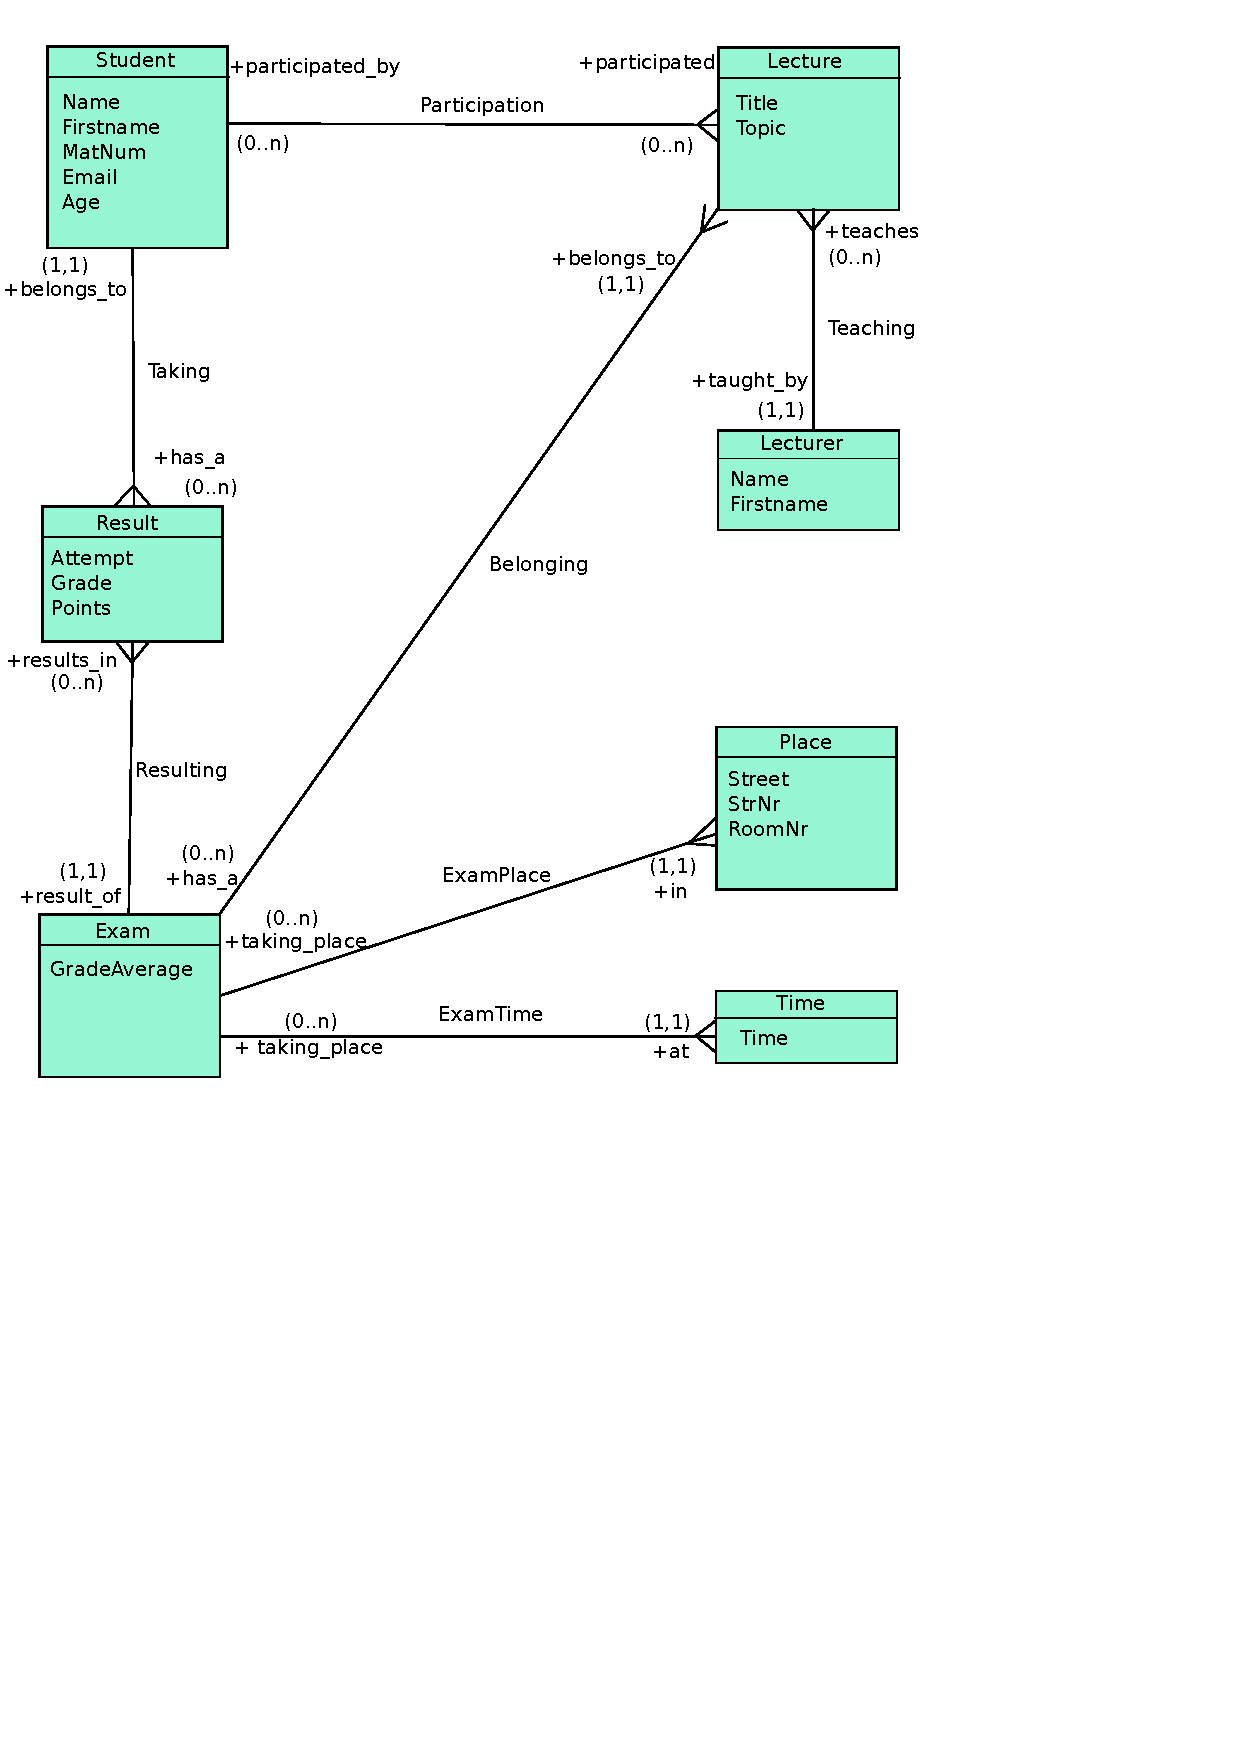
\includegraphics[trim= 0 320 120 0,scale=0.7, clip=true]{\curryhome/currytools/currypp/Docs/diagram.pdf}
\end{center}
\caption{A simple entity-relationship diagram for university lectures \cite{HanusKrone17EPTCS}}
\label{fig:erd}
\end{figure*}

Instead of requiring the use of soem graphical ER modeling tool,
ERDs must be specified in textual form as a Curry data term,
see also \cite{BrasselHanusMueller08PADL}.
In this representation, an ERD has a name, which is also used
as the module name of the generated Curry code,
lists of entities and relationships:
%
\begin{curry}
data ERD = ERD String [Entity] [Relationship]
\end{curry}
%
Each entity consists of a name and a list of attributes, where
each attribute has a name, a domain, and specifications
about its key and null value property:
\begin{curry}
data Entity = Entity String [Attribute]

data Attribute = Attribute String Domain Key Null

data Key = NoKey | PKey | Unique

type Null = Bool

data Domain = IntDom             (Maybe Int)
            | FloatDom           (Maybe Float)
            | CharDom            (Maybe Char)
            | StringDom          (Maybe String)
            | BoolDom            (Maybe Bool)
            | DateDom            (Maybe ClockTime)
            | UserDefined String (Maybe String)
            | KeyDom String   -- later used for foreign keys
\end{curry}
%
Thus, each attribute is part of a primary key (\code{PKey}),
unique (\code{Unique}), or not a key (\code{NoKey}).
Furthermore, it is allowed that specific attributes can have null values, i.e.,
can be undefined. The domain of each attribute is one of the standard
domains or some user-defined type. In the latter case, the
first argument of the constructor \code{UserDefined}
is the qualified type name used in the Curry application program.
For each kind of domain, one can also have a default value
(modeled by the \code{Maybe} type).
The constructor \code{KeyDom} is not necessary to represent ERDs
but it is internally used to transform complex ERDs
into relational database schemas.

Finally, each relationship has a name and a list of connections
to entities (\code{REnd}), where each connection has the name
of the connected entity, the role name of this connection,
and its cardinality as arguments:
\begin{curry}
data Relationship = Relationship String [REnd]

data REnd = REnd String String Cardinality

data Cardinality = Exactly Int | Between Int MaxValue

data MaxValue = Max Int | Infinite
\end{curry}
The cardinality is either a fixed integer or a range between two
integers (where \code{Infinite} as the upper bound represents an
arbitrary cardinality).
For instance, the simple-complex (1:n) relationship \code{Teaching}
in Fig.\ref{fig:erd} can be represented by
the term
\begin{curry}
Relationship "Teaching"
             [REnd "Lecturer" "taught_by" (Exactly 1),
              REnd "Lecture" "teaches"    (Between 0 Infinite)]
\end{curry}
%
The \CYS library \code{Database.ERD} contains the ER datatypes
described above. Thus, the specification of the
conceptual database model must be a data term of type
\code{Database.ERD.ERD}.
%
\begin{figure}[t]
\begin{curry}
 ERD "Uni"
   [Entity "Student"
           [Attribute "Name" (StringDom Nothing) NoKey False,
            Attribute "Firstname" (StringDom Nothing) NoKey False,
            Attribute "MatNum" (IntDom Nothing) Unique False,
            Attribute "Email" (StringDom Nothing) Unique False,
            Attribute "Age" (IntDom Nothing) NoKey True],
    Entity "Lecture"
           [Attribute "Title" (StringDom Nothing) NoKey False,
            Attribute "Topic" (StringDom Nothing) NoKey True],
    Entity "Lecturer"
           [Attribute "Name" (StringDom Nothing) NoKey False,
            Attribute "Firstname" (StringDom Nothing) NoKey False],
    Entity "Place"
           [Attribute "Street" (StringDom Nothing) NoKey False,
            Attribute "StrNr" (IntDom Nothing) NoKey False,
            Attribute "RoomNr" (IntDom Nothing) NoKey False], 
    Entity "Time"
           [Attribute "Time" (DateDom Nothing) Unique False],
    Entity "Exam"
           [Attribute "GradeAverage" (FloatDom Nothing) NoKey True],
    Entity "Result"
           [Attribute "Attempt" (IntDom Nothing) NoKey False,  
            Attribute "Grade" (FloatDom Nothing) NoKey True,
            Attribute "Points" (IntDom Nothing) NoKey True]]
   [Relationship "Teaching"
                 [REnd "Lecturer" "taught_by" (Exactly 1),
                  REnd "Lecture" "teaches" (Between 0 Infinite)],
    Relationship "Participation"
                 [REnd "Student" "participated_by" (Between 0 Infinite),
                  REnd "Lecture" "participates" (Between 0 Infinite)],
    Relationship "Taking"
                 [REnd "Result" "has_a" (Between 0 Infinite),
                  REnd "Student" "belongs_to" (Exactly 1)],
    Relationship "Resulting"
                 [REnd "Exam" "result_of" (Exactly 1),
                  REnd "Result" "results_in" (Between 0 Infinite)],
    Relationship "Belonging"
                 [REnd "Exam" "has_a" (Between 0 Infinite),
                  REnd "Lecture" "belongs_to" (Exactly 1)],
    Relationship "ExamDate"
                 [REnd "Exam" "taking_place" (Between 0 Infinite),
                  REnd "Time" "at" (Exactly 1)],
    Relationship "ExamPlace"
                 [REnd "Exam" "taking_place" (Between 0 Infinite),
                  REnd "Place" "in" (Exactly 1)]]
\end{curry}
\caption{The ER data term specification of Fig.~\ref{fig:erd}\label{fig:erdterm}}
\end{figure}
Figure~\ref{fig:erdterm} on (page~\pageref{fig:erdterm})
shows the complete ER data term specification
corresponding to the ERD of Fig.~\ref{fig:erd}.

Such a data term specification should be stored in Curry program file
as an (exported!) top-level operation type \code{ERD}.
If our example term is defined as a constant in the Curry program
\code{UniERD.curry}, then one has to use the tool \ccode{erd2curry}
(see Sect.~\ref{sec-erd2curry})
to process the ER model so that it can be used
in SQL statements. This tool is invoked with the parameter
\ccode{--cdbi},
the (preferably absolute) file name of the SQLite database,
and the name of the Curry program containing the ER specification.
If the SQLite database file does not exist, it will be initialized by the tool.
In our example, we execute the following command
(provided that the tool \code{erd2curry} is already installed,
see Sect.~\ref{sec-erd2curry}):
%
\begin{curry}
> erd2curry --db `pwd`/Uni.db --cdbi UniERD.curry
\end{curry}
%
This initializes the SQLite database \code{Uni.db}
and performs the following steps:
%
\begin{enumerate}
\item 
The ER model is transformed into tables of a relational database,
i.e., the relations of the ER model are either represented
by adding foreign keys to entities (in case of (0/1:1) or (0/1:n) relations)
or by new entities with the corresponding relations
(in case of complex (n:m) relations).
\item
A new Curry module \code{Uni\us{}CDBI} is generated.
It contains the definitions of
entities and relationships as Curry data types.
Since entities are uniquely identified via a database key,
each entity definition has, in addition to its attributes, this key as the
first argument.
For instance, the following definitions are generated
for our university ERD (among many others):
%
\begin{curry}
data StudentID = StudentID Int$\listline$
data Student = Student StudentID String String Int String Int$\listline$
-- Representation of n:m relationship Participation:
data Participation = Participation StudentID LectureID
\end{curry}
%
Note that the two typed foreign key columns (\code{StudentID}, \code{LectureID})
ensures a type-safe handling of foreign-key constraints.
These entity descriptions are relevant for SQL queries
since some queries (e.g., those that do not project on particular database
columns) return lists of such entities.
Moreover, the generated module contains useful getter and setter functions
for each entity.
Other generated operations, like entity description and definitions
of their columns, are not relevant for the programming
but only used for the translation of SQL statements.
\item
Finally, an \emph{info file} \code{Uni_SQLCODE.info} is created.
It contains information about all entities,
attributes and their types, and relationships.
This file is used by the SQL parser and translator of the
Curry preprocessor to type check the SQL statements
and generate appropriate Curry library calls.
\end{enumerate}


\subsubsection{SQL Statements as Integrated Code}

After specifying and processing the ER model of the database,
one can write SQL statement in their standard syntax
as integrated code (marked by the prefix \ccode{sql}) in Curry programs.
For instance, to retrieve all students from the database, one
can define the following SQL query:
%
\begin{curry}
allStudents :: IO (SQLResult [Student])
allStudents = ``sql Select * From Student;''
\end{curry}
%
Since database accesses might produce errors,
the result of SQL statements is always of type
\ccode{SQLResult $\tau$}, where \code{SQLResult} is a type synonym
defined in the \CYS library \code{Database.CDBI.Connection}:
%
\begin{curry}
type SQLResult a = Either DBError a
\end{curry}
%
This library defines also an operation
%
\begin{curry}
fromSQLResult :: SQLResult a -> a
\end{curry}
%
which returns the retrieved database value or raises a run-time error.
Hence, if one does not want to check the occurrence of database errors
immediately, one can also define the above query as follows:
%
\begin{curry}
allStudents :: IO [Student]
allStudents = liftIO fromSQLResult ``sql Select * From Student;''
\end{curry}
%
In order to select students with an age between 20 and 25,
one can put a condition as usual:
%
\begin{curry}
youngStudents :: IO (SQLResult [Student])
youngStudents = ``sql Select * From Student
                      Where Age between 18 and 21;''
\end{curry}
%
Usually, one wants to parameterize queries over some values
computed by the context of the Curry program.
Therefore, one can embed Curry expressions instead of concrete
values in SQL statements by enclosing them in curly brackets:
%
\begin{curry}
studAgeBetween :: Int -> Int -> IO (SQLResult [Student])
studAgeBetween min max =
  ``sql Select * From Student
        Where Age between {min} and {max};''
\end{curry}
%
Instead of retrieving complete entities (database tables),
one can also project on some attributes (database columns)
and one can also order them with the usual \ccode{Order By} clause:
%
\begin{curry}
studAgeBetween :: Int -> Int -> IO (SQLResult [(String,Int)])
studAgeBetween min max =
  ``sql Select Name, Age
        From Student Where Age between {min} and {max}
        Order By Name Desc;''
\end{curry}
%
In addition to the usual SQL syntax, one can also
write conditions on relationships between entities.
For instance, the following code will be accepted:
%
\begin{curry}
studGoodGrades :: IO (SQLResult [(String, Float])
studGoodGrades = ``sql Select Distinct s.Name, r.Grade 
                       From Student as s, Result as r
                       Where Satisfies s has_a r And r.Grade < 2.0;''
\end{curry}
%
This query retrieves a list of pairs containing the
names and grades of students having a grade better than \code{2.0}.
This query is beyond pure SQL since it also includes
a condition on the relation \code{has\us{}a} specified in the ER model
(\ccode{Satisfies s has\us{}a r}).

The complete SQL syntax supported by the Curry preprocessor
is shown in Appendix~\ref{app:sqlsyntax}.
More details about the implementation of this
SQL translator can be found in \cite{HanusKrone17EPTCS,Krone15}.


%%%%%%%%%%%%%%%%%%%%%%%%%%%%%%%%%%%%%%%%%%%%%%%%%%%%%%%%%%%%%%%%%%%%%%%%%%%%
\subsection{Sequential Rules}

If the Curry preprocessor is called with the option
\ccode{seqrules}, then all rules in the Curry module are
interpreted in a sequential manner, i.e., a rule is applied only
if all previous rules defining the same operation are not applicable,
either because the left-hand side's pattern does not match
or the condition is not satisfiable.
The idea and detailed semantics of
sequential rules are described in \cite{AntoyHanus14}.
Sequential rules are useful and preferable over
rules with multiple guards if the patterns are non-trivial
(e.g., functional patterns) or the condition involve complex
constraints.

As a simple example, the following module defines
a lookup operation in association lists by a functional pattern.
Due to the sequential rule strategy,
the second rule is applied only if there is no appropriate
key in the association list:
%
\begin{curry}
{-# OPTIONS_CYMAKE -F --pgmF=currypp --optF=seqrules #-}

mlookup key (_ ++ [(key,value)] ++ _) = Just value
mlookup _   _                         = Nothing 
\end{curry}


%%%%%%%%%%%%%%%%%%%%%%%%%%%%%%%%%%%%%%%%%%%%%%%%%%%%%%%%%%%%%%%%%%%%%%%%%%%%
\subsection{Default Rules}

An alternative to sequential rules are default rules, i.e.,
these two options cannot be simultaneously used.
Default rules are activated by the preprocessor option
\ccode{defaultrules}.
In this case, one can add to each operation a default rule.
A default rule for a function $f$ is defined as a rule
defining the operation \ccode{$f$'default} (this mechanism
avoids any language extension for default rules).
A default rule is applied only if no ``standard'' rule is
applicable, either because the left-hand sides' pattern do not match
or the conditions are not satisfiable.
The idea and detailed semantics of
default rules are described in \cite{AntoyHanus16PADL}.

Default rules are preferable over the sequential rule selection
strategy since they have a better operational behavior.
This is due to the fact that the test for the application
of default rules is done with the same (sometimes optimal)
strategy than the selection of standard rules.
Moreover, default rules provide a similar power than sequential rules,
i.e., they can be applied if the standard rules have
complex (functional) patterns or complex conditions.

As a simple example, we show the implementation of the
previous example for sequential rules with a default rule:
%
\begin{curry}
{-# OPTIONS_CYMAKE -F --pgmF=currypp --optF=defaultrules #-}

mlookup key (_ ++ [(key,value)] ++ _) = Just value
mlookup'default _   _                 = Nothing 
\end{curry}
%
Default rules are often a good replacement for ``negation as failure''
used in logic programming.
For instance, the following program defines a solution
to the $n$-queens puzzle, where the default rule is useful
since it is easier to characterize the unsafe positions
of the queens on the chessboard (see the first rule of \code{safe}):
%
\begin{curry}
{-# OPTIONS_CYMAKE -F --pgmF=currypp --optF=defaultrules #-}

import Combinatorial(permute)
import Integer(abs)

-- A placement is safe if two queens are not in a same diagonal:
safe (_++[x]++ys++[z]++_) | abs (x-z) == length ys + 1 = failed
safe'default xs = xs

-- A solution to the n-queens puzzle is a safe permutation:
queens :: Int -> [Int]
queens n = safe (permute [1..n])
\end{curry}


%%%%%%%%%%%%%%%%%%%%%%%%%%%%%%%%%%%%%%%%%%%%%%%%%%%%%%%%%%%%%%%%%%%%%%%%%
\subsection{Contracts}

Contracts are annotations in Curry program to specify the
intended meaning and use of operations by other operations
or predicates expressed in Curry.
The idea of using contracts for the development
of reliable software is discussed in \cite{AntoyHanus12PADL}.
The Curry preprocessor supports dynamic contract checking
by transforming contracts, i.e., specifications and
pre-/postconditions, into assertions that are checked
during the execution of a program.
If some contract is violated, the program terminates
with an error.

The transformation of contracts into assertions is described
in \cite{AntoyHanus12PADL}.
Note that only strict assertion checking is supported
at the moment.
Strict assertion checking might change the operational behavior
of the program.
The notation of contracts has been shortly introduced
in Section~\ref{sec:currycheck:contracts}.
To transform such contracts into assertions,
one has to use the option \ccode{contracts} for the preprocessor.

As a concrete example, consider an implementation of quicksort
with a postcondition and a specification as shown in
Section~\ref{sec:currycheck:contracts}
(where the code for \code{sorted} and \code{perm} is not shown here):
%
\begin{curry}
{-# OPTIONS_CYMAKE -F --pgmF=currypp --optF=contracts #-}

$\ldots$

-- Trivial precondition:
sort'pre xs = length xs >= 0

-- Postcondition: input and output lists should have the same length
sort'post xs ys = length xs == length ys

-- Specification:
-- A correct result is a permutation of the input which is sorted.
sort'spec :: [Int] -> [Int]
sort'spec xs | ys == perm xs && sorted ys = ys  where ys free

-- A buggy implementation of quicksort:
sort :: [Int] -> [Int]
sort []     = []
sort (x:xs) = sort (filter (<x) xs) ++ [x] ++ sort (filter (>x) xs)
\end{curry}
%
If this program is executed, the generated assertions report
a contract violation for some inputs:
%
\begin{curry}
Quicksort> sort [3,1,4,2,1]
Postcondition of 'sort' (module Quicksort, line 27) violated for:
[1,2,1] -> [1,2]

ERROR: Execution aborted due to contract violation!
\end{curry}

%  LocalWords:  preprocessor


%%% Local Variables: 
%%% mode: latex
%%% TeX-master: "../../../docs/src/manual"
%%% End: 
